\documentclass[compress]{beamer}

%--------------------------------------------------------------------------
% Common packages
%--------------------------------------------------------------------------
\usepackage[english]{babel}
\usepackage{pgfpages} % required for notes on second screen
\usepackage{graphicx}
\usepackage{subfigure}
\usepackage{multicol}
\usepackage[normalem]{ulem}

\usepackage{tabularx,ragged2e}
\usepackage{booktabs}
\usepackage{marvosym}

%--------------------------------------------------------------------------
% Load theme
%--------------------------------------------------------------------------
\usetheme{hri}

\usepackage{tikz}
\usetikzlibrary{shapes,fpu,fit,calc,mindmap,backgrounds,positioning,svg.path}

\tikzset{
    invisible/.style={opacity=0},
  visible on/.style={alt={#1{}{invisible}}},
  alt/.code args={<#1>#2#3}{%
      \alt<#1>{\pgfkeysalso{#2}}{\pgfkeysalso{#3}} % \pgfkeysalso doesn't change the path
  },
}

\graphicspath{{figs/}}


%--------------------------------------------------------------------------
% General presentation settings
%--------------------------------------------------------------------------
\title{robots in the classroom}
\subtitle{to be or not to be social?}
\date{Cognovo Symposium: Group Creativity and Education -- {\bf 26th Jan 2017}}
\author{Séverin Lemaignan}
\institute{Centre for Robotics and Neural Systems {\bf Plymouth University} \\
        CHILI Lab {\bf EPFL}}

%--------------------------------------------------------------------------
% Notes settings
%--------------------------------------------------------------------------
%\setbeameroption{show notes on second screen}
%\setbeameroption{hide notes}

\begin{document}

\licenseframe{https://github.com/severin-lemaignan/presentation-cognitive-robotics}
\maketitle

%%%%%%%%%%%%%%%%%%%%%%%%%%%%%%%%%%%%%%%%%%%%%%%%%%%%%%%%%%%%%%%%%%%%%%%%%%%%%%%
%%%%%%%%%%%%%%%%%%%%%%%%%%%%%%%%%%%%%%%%%%%%%%%%%%%%%%%%%%%%%%%%%%%%%%%%%%%%%%%
%%%%%%%%%%%%%%%%%%%%%%%%%%%%%%%%%%%%%%%%%%%%%%%%%%%%%%%%%%%%%%%%%%%%%%%%%%%%%%%

\imageframe{croquignole.jpg}

\begin{frame}{Social or not Social?}
    \begin{center}
        \resizebox{\linewidth}{!}{
            \begin{tikzpicture}[>=latex]
                \node[double arrow,draw,fill=hriSec1] (spec) {\bf Interaction spectrum};
                \node<1>[left=of spec] {Non-social};
                \node<2>[left=of spec] {\bf Cellulo};
                \node<1>[right=of spec] {Social};
                \node<2>[right=of spec] {\bf CoWriter};
            \end{tikzpicture}
        }
    \end{center}
\end{frame}

%%%%%%%%%%%%%%%%%%%%%%%%%%%%%%%%%%%%%%%%%%%%%%%%%%%%%%
%%%%%%%%%%%%%%%%%%%%%%%%%%%%%%%%%%%%%%%%%%%%%%%%%%%%%%
%% Cellulo
%%%%%%%%%%%%%%%%%%%%%%%%%%%%%%%%%%%%%%%%%%%%%%%%%%%%%%
%%%%%%%%%%%%%%%%%%%%%%%%%%%%%%%%%%%%%%%%%%%%%%%%%%%%%%

\begin{frame}{Non-social interaction}
    What is the most effective learning tool in a classroom?

    \begin{center}
        \includegraphics<2>[width=0.8\linewidth]{cellulo/pencil}
    \end{center}
\end{frame}

\imageframe[caption=Pens and paper are pervasive...]{cellulo/classroom}
\imageframe[caption=...so should be the robots]{cellulo/classroom-withcellulo}

{
    \paper{\"Ozg\"ur, Lemaignan et al. {\bf Cellulo: Versatile Handheld Robots
    for Education} -- HRI 2017}
 \begin{frame}{Cellulo: design principles}

     \begin{itemize}
         \item<1-> {\bf ubiquitous}: a pervasive yet unremarkable tool
             that blend into the daily learning routine; has to be reliable (\ie
             trustworthy), readily replaceable (\ie cheap, no affective bonding), intuitive (\ie few
             simple affordances)

         \item<2-> {\bf versatile}: applicable to a broad range of learning
             scenarios; the robots’ hardware, appearance and interaction
             modalities must not imply or be constrained to specific use cases

         \item<3-> {\bf practical}: to gain field
             acceptance in the classrooms, educative robots must critically
             represent a net educative gain and must not incur higher
             workload for the teachers
     \end{itemize}

        %\badge{europe_epfl}
 \end{frame}
}

\begin{frame}{How does it look like?}
    \begin{center}
        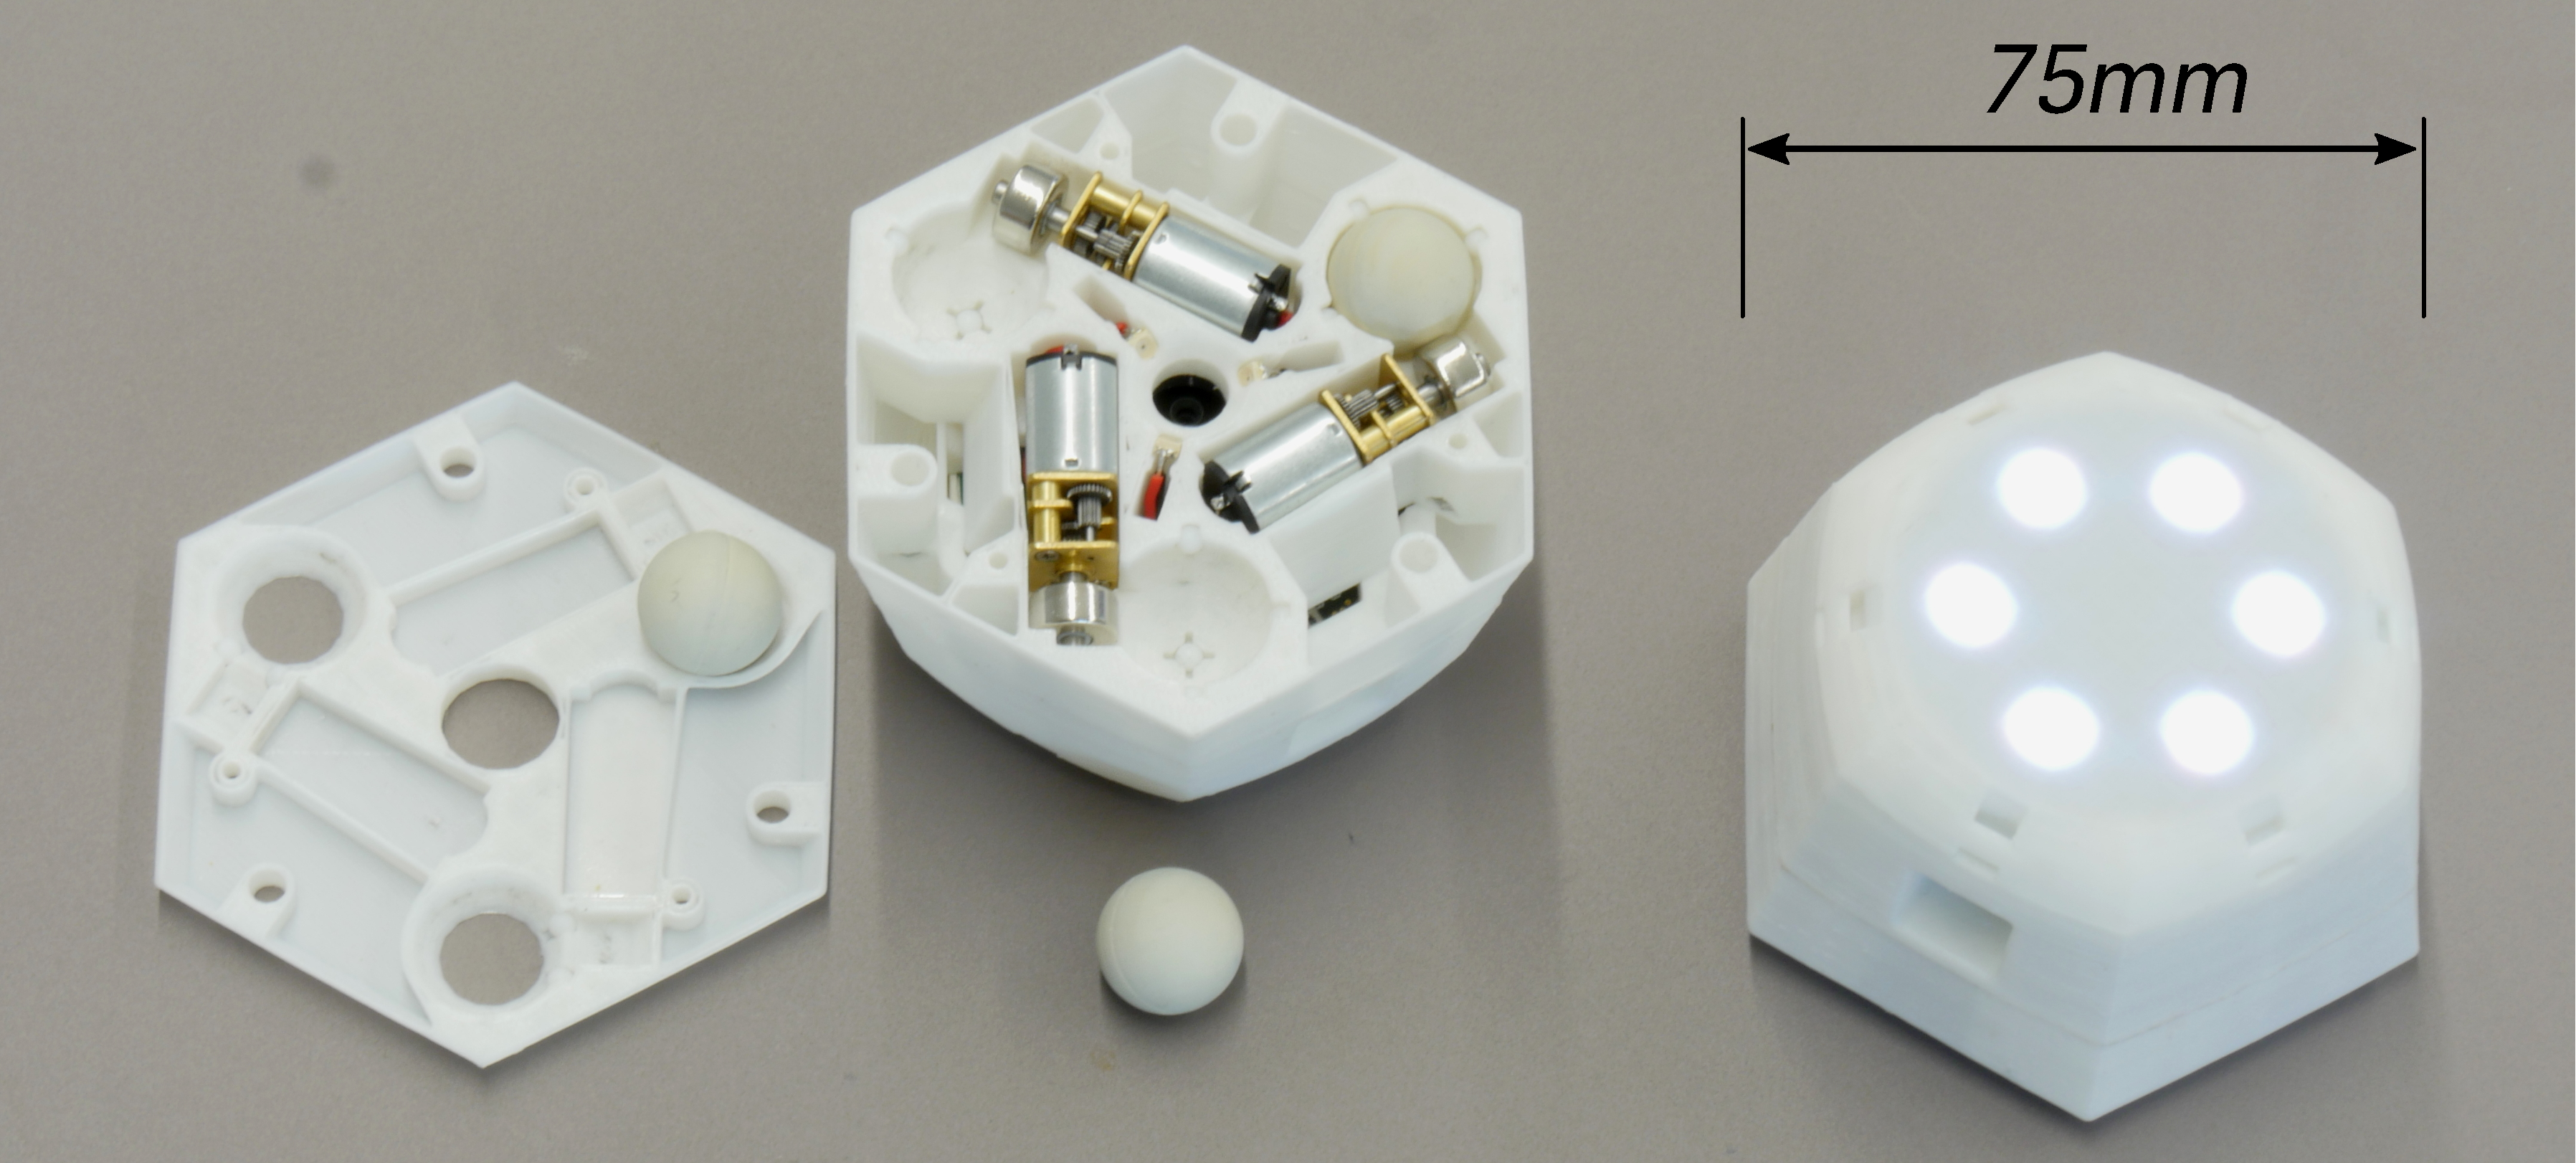
\includegraphics[width=0.8\linewidth]{cellulo/hardware-design}
    \end{center}
    \begin{itemize}
        \item Omnidirectional
        \item Haptic feedback + tactile RGB LED buttons 
        \item Bluetooth
        \item Accurate self-localisation
        \item<2> Affordable (prototype: \pounds100)
    \end{itemize}
    %\badge{europe_epfl}
\end{frame}

\videoframe[0.56]{figs/cellulo/cellulo-swarm-demo.mp4}

\begin{frame}{Interaction with the paper}
    %\badge{europe_epfl}
    Critically, Cellulo is meant as an {\bf interaction between the
    (classroom-friendly) paper and the robots}.

    \pause

    Achieved through a {\bf paper-based self-localisation system}

    \begin{center}
        \includegraphics<3>[width=0.8\linewidth]{cellulo/treasure-game-1}
        \includegraphics<4>[width=\linewidth]{cellulo/treasure-game-2}
    \end{center}

    \only<5>{

        \begin{itemize}
            \item even more than 'classroom-friendly', paper is 'teacher-friendly'
            \item easy to manipulate, copy, print, cutout, dispose...
            \item unique activity IDs: drop the robots onto the sheet, it
                recognizes the activity
        \end{itemize}
    }

\end{frame}

\imageframe[color=black,caption=Concept 1: chemistry]{cellulo/concept-molecules}
\imageframe[color=black,caption=Concept 2: solar system]{cellulo/concept-solar-system}

\begin{frame}{Interaction Design space}
    \begin{center}
        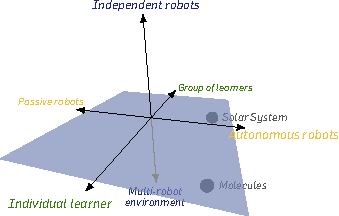
\includegraphics[width=0.8\linewidth]{cellulo/interaction-space}
    \end{center}
    %\badge{europe_epfl}
\end{frame}

 \begin{frame}[plain]{}
     ...at the other end of the spectrum...
 \end{frame}


 %%%%%%%%%%%%%%%%%%%%%%%%%%%%%%%%%%%%%%%%%%%%%%%%%%%%%%
 %%%%%%%%%%%%%%%%%%%%%%%%%%%%%%%%%%%%%%%%%%%%%%%%%%%%%%
 %%%%%%%%%%%%%%%%%%%%%%%%%%%%%%%%%%%%%%%%%%%%%%%%%%%%%%
 %% CoWriter
 %%%%%%%%%%%%%%%%%%%%%%%%%%%%%%%%%%%%%%%%%%%%%%%%%%%%%%

\imageframe[color=black]{cowriter/social-learning}

\imageframe{cowriter/joe1}
\imageframe{cowriter/joe2}
\imageframe[color=black]{cowriter/diego-writing}


\begin{frame}{Robots?}
    %\badge{europe_epfl}
    \begin{itemize}
        \item<1-> Robots do not know how to write!
        \item<2-> Learning by teaching
        \item<3-> (nice side-effect: we can adapt to each child and each disabilities)
    \end{itemize}
\end{frame}

\imageframe[color=black]{cowriter/diego-correct}

\begin{frame}[plain]{}
    \centering
    Mind modelling is {\bf mutual}

    We can take advantage of it in human-robot interaction at fundamental levels

\end{frame}

\begin{frame}{Cognitive Engagement and Meta-cognition}
    \video{0.55\textwidth}{figs/cowriter/cowriter-session1_3minExcerpt_1x.mp4}

    \begin{flushright}
        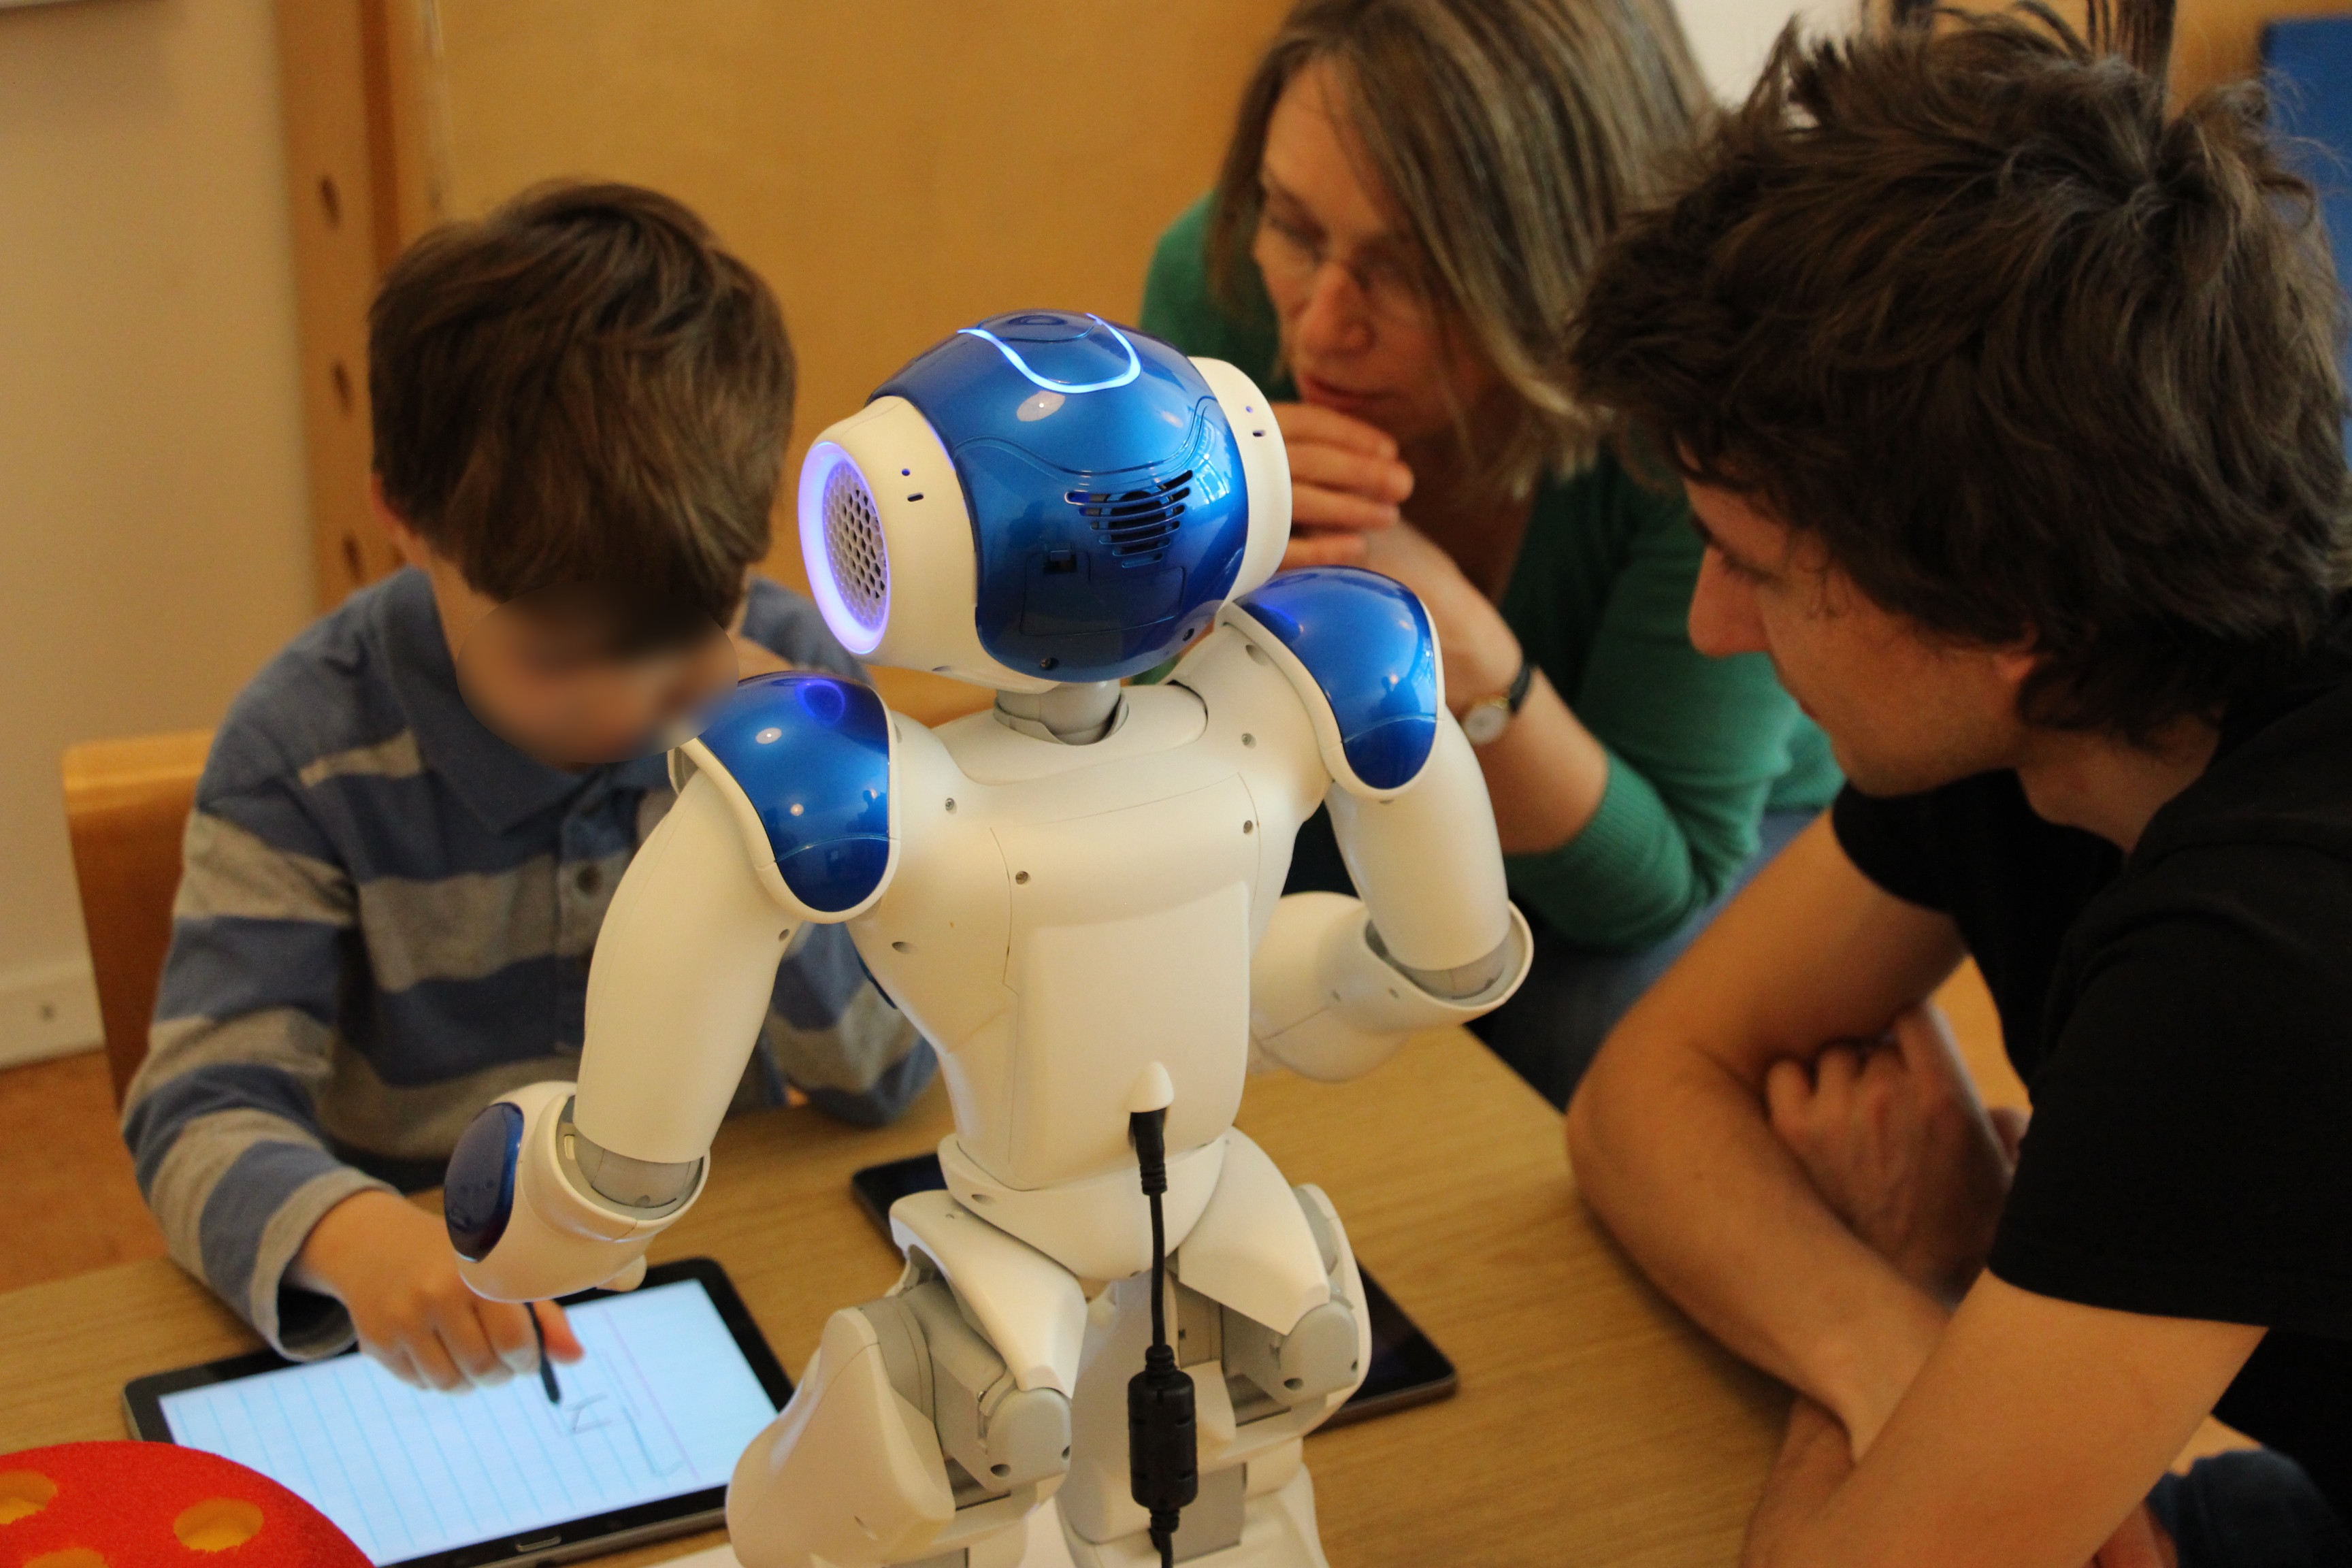
\includegraphics[width=0.5\textwidth]{cowriter/henry}
    \end{flushright}

\end{frame}

\begin{frame}{Learning from demonstration}
    \begin{center}
    
\includegraphics[width=0.8\textwidth]{cowriter/learningSdemo.png}
    \end{center}
\end{frame}

%\begin{frame}{Technical Challenges}
%    %\badge{europe_epfl}
%    \begin{itemize}
%        \item<1-> Get a child-proof robot to write...
%        \item<2-> ...badly...
%        \item<3-> Make it able to learn...
%        \item<4-> ...with the help of children
%    \end{itemize}
%\end{frame}
%
%
%\begin{frame}{CoWriter implementation}
%    \centering
%
%    \only<1>{
%        \video{0.8\textwidth}{figs/cowriter/nao-tablet-demo.mp4}
%    }
%
%    \only<2>{
%        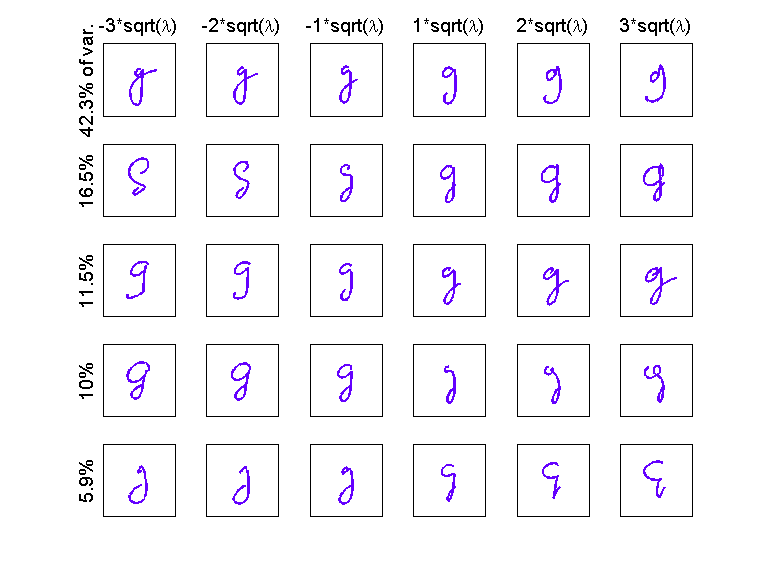
\includegraphics[width=0.8\textwidth]{cowriter/cowriter-g.png}
%    }
%
%    %\badge{europe_epfl}
%\end{frame}

\begin{frame}{Before -- After}
    \begin{center}
        \only<1-2>{
        \includegraphics[width=0.43\linewidth]{cowriter/lettre-base}
        \uncover<2>{
            \hspace{1cm}%
        \includegraphics[width=0.43\linewidth]{cowriter/lettre-final}
        }
        }
        \only<3>{
        \includegraphics[width=0.43\linewidth]{cowriter/lettre-base-highlight}
            \hspace{1cm}%
        \includegraphics[width=0.43\linewidth]{cowriter/lettre-final-highlight}
        }
    \end{center}
        %\badge{europe_epfl}
\end{frame}

\begin{frame}{Learning to draw a 5}
    \begin{center}
        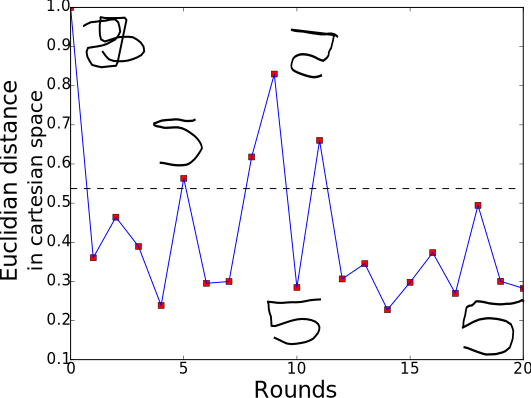
\includegraphics[width=0.8\linewidth]{cowriter/henry5}
    \end{center}
\end{frame}

{
    \paper{Lemaignan et al. {\bf Learning by Teaching a Robot: The Case of Handwriting} -- Robotics and Automation Magazine 2016}
\begin{frame}{The Robot as a Social Agent}
    \begin{itemize}
        \item<+-> {\bf The robot as a cognitive agent is key here}
            \begin{itemize}
                \item Protégé effect
                \item metacognition
            \end{itemize}
        \item<+-> \textbf{New role}: not a 'tool to teach robotics', not a facilitator
        \item<+-> (note: a tool for the teacher vs a social agent for the child!)
        \item<+-> Could we replace it by someone else? Not easily
    \end{itemize}

\end{frame}
}


%\imageframe{cowriter/cowriter-fsm.png}

%%%%%%%%%%%%%%%%%%%%%%%%%%%%%%%%%%%%%%%%%%%%%%%%%%%%%%%%%%%%%%%%%%%%%%%%%%%%%%%%%%
%%%%%%%%%%%%%%%%%%%%%%%%%%%%%%%%%%%%%%%%%%%%%%%%%%%%%%%%%%%%%%%%%%%%%%%%%%%%%%%%%

%%%%%%%%%%%%%%%%%%%%%%%%%%%%%%%%%%%%%%%%%%%%%%%%%%%%%%%%%%%%%%%%%%%%%%%%%%%%%%%%
%%%%%%%%%%%%%%%%%%%%%%%%%%%%%%%%%%%%%%%%%%%%%%%%%%%%%%%%%%%%%%%%%%%%%%%%%%%%%%%%%


{
\fullbackground{ranger/ranger_funny_glasses}
\begin{frame}[plain]

    \vspace{8cm}

\setbeamercolor{hriSec1Demo}{fg=white}
\begin{beamercolorbox}[wd=\linewidth,ht=6ex,dp=0.7ex]{hriSec1Demo}
        \Large
        So? Social or not social?\\[2em]
        \normalsize
    \textbf{Thank you!}\\
    \scriptsize
    Séverin Lemaignan\\
    Portland Square A216 -- {\tt severin.lemaignan@plymouth.ac.uk}
\end{beamercolorbox}
    \vfill
\end{frame}
}

%%%%%%%%%%%%%%%%%%%%%%%%%%%%%%%%%%%%%%%%%%%%%%%%%%%%%%%%%%%%%%%%%%%%%%%%%%%%%%%%%
%%%%%%%%%%%%%%%%%%%%%%%%%%%%%%%%%%%%%%%%%%%%%%%%%%%%%%%%%%%%%%%%%%%%%%%%%%%%%%%%%

\section{Child-robot interaction on the practical side}

\imageframe{croquignole.jpg}

{
\paper{Lemaignan, Hosseini, Dillenbourg {\bf pyRobots: a Toolset for Robot Executive Control} -- IROS 2015}
\begin{frame}{}
    \centering
    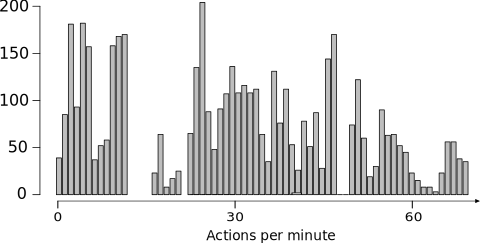
\includegraphics[width=0.8\textwidth]{actions-croquignole.pdf}

    \begin{multicols}{3}
\scriptsize
{\tt lightbar} \\
{\tt on\_toy\_added} \\
{\tt move} \\
{\tt background\_blink} \\
{\tt undock} \\
{\tt pulse\_row} \\
{\tt blink} \\
{\tt on\_lolette} \\
{\tt placeeyes} \\
{\tt on\_bumped} \\
{\tt up\_down\_row} \\
{\tt wakeup} \\
{\tt look\_at\_caresses} \\
{\tt on\_toy\_removed} \\
{\tt sneak\_in} \\
{\tt on\_lolette\_removed} \\
{\tt fall\_asleep} \\
{\tt look\_at\_lolette} \\
{\tt active\_wait} \\
{\tt closeeyes} \\
{\tt lightpattern} \\
{\tt turn} \\
{\tt idle} \\
{\tt playsound} \\
{\tt blush}

    \end{multicols}
\end{frame}
}



%%%%%%%%%%%%%%%%%%%%%%%%%%%%%%%%%%%%%%%%%%%%%%%%%%%%%%%%%%%%%%%%%%%%%%%%%%%%%%%%%
\subsection{With-me-ness}

\begin{frame}{}

    \begin{center}

        Can we make the analysis of child-robot interaction {\bf practical}?

        \begin{itemize}
            \item (surface) engagement
            \item cognitive perception/anthropomorphism
            \item child speech recognition
        \end{itemize}

    \end{center}

\end{frame}


\imageframe[color=black]{realSetup}
\imageframe[color=black]{no-attention}

\begin{frame}{Expected focus}

    \centering

    Example for the CoWriter task:

        \begin{multicols}{2}
           \scriptsize 
           \begin{tabular}{p{2.5cm}p{2.5cm}}
            \toprule
            {\bf Interaction Phase} & {\bf Expected targets} \\
            \midrule
            Presentation & {\sf robot} \\ 
            \midrule
            Waiting for word & {\sf secondary tablet} \\ 
            \midrule
            Writing word & {\sf tablet}\newline {\sf robot} \\ 
            \midrule
            Waiting for feedback & {\sf tablet}\newline {\sf secondary tablet} \\ 
            \midrule
            Story telling & {\sf robot} \\ 
            \midrule
            Bye & {\sf robot} \\ 
            \bottomrule
        \end{tabular}

            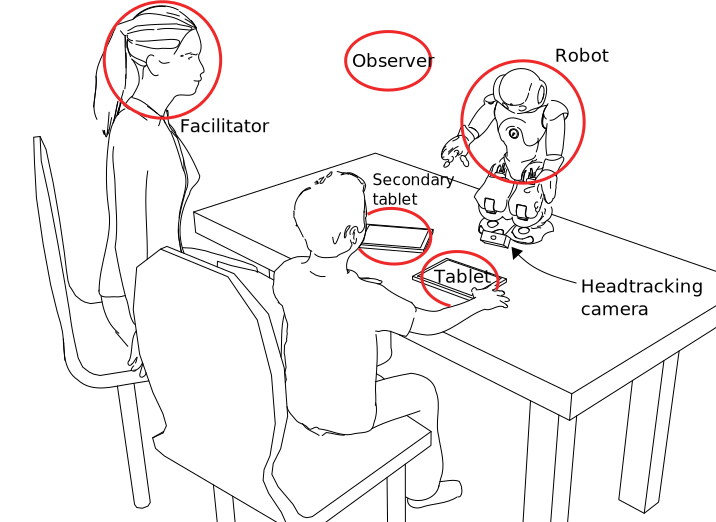
\includegraphics[width=0.95\columnwidth]{experimental_setup}
        \end{multicols}

\end{frame}



\imageframe[color=black]{head_pose_real_world}

{
\paper{Lemaignan et al. {\bf From Real-time Attention Assessment to “With-me-ness” in Human-Robot Interaction} -- HRI 2016}
\fullbackground[scale=0.95]{with-me-ness-robot}

\begin{frame}{With-me-ness}
        %\badge{europe_epfl}
\end{frame}
}

\begin{frame}{With-me-ness is...}

    {\bf With-me-ness is...}

    \begin{itemize}
        \item An {\bf objective} \& {\bf quantitative} precursor of engagement...
        \item ...based on matching the {\bf user's focus of attention} with a set of
            {\bf prior expectations}
        \item Can be computed {\bf on-line} by the robot...
        \item ...and {\bf sensitive to} the (task-dependent) {\bf set of
            expectations}
        \item $\Rightarrow$ {\bf relative} metric!
    \end{itemize}

    \centering

\end{frame}


%%%%%%%%%%%%%%%%%%%%%%%%%%%%%%%%%%%%%%%%%%%%%%%%%%%%%%%%%%%%%%%%%%%%%%%%%%%%%%%%%

{
    \paper{Lemaignan, Fink, Mondada, Dillenbourg {\bf You're Doing
    It Wrong! Studying Unexpected Behaviors in CRI} ICSR
    2015}
\begin{frame}{Constructs for Cognitive Perception analysis}
\tiny
    \begin{multicols}{2}
    \begin{table}[]
        \begin{tabularx}{\linewidth}{p{0.9\linewidth}}

    \toprule
    {\bf Expectations} \tabularnewline
    \midrule
    \emph{How do you imagine a robot?} \tabularnewline
    \emph{What could it look like?} \tabularnewline
    \emph{Have you ever seen a robot before?} \tabularnewline

    %%
    \toprule
    {\bf Impression} \tabularnewline
    \midrule


    \emph{When you first saw R, what did you think?} \tabularnewline
    \emph{Is R a robot? How do you know?} \tabularnewline
    \emph{Did you expect R would come over to you when you call it?} \tabularnewline
    \emph{What happened when you put the domino in the box?} \tabularnewline

    %%
    \toprule
    {\bf Ascribe intention} \tabularnewline
    \midrule


    \emph{Do you think R could go out the door all by itself?} \tabularnewline	
    \emph{Does R always obey / come over to you?} \tabularnewline
    \emph{Could R do something silly?} \tabularnewline
    \emph{Why did R not come over to you when you called it?} \tabularnewline

            \bottomrule
        \end{tabularx}
        \label{tab:options}
    \end{table}

    \begin{table}[]
        \begin{tabularx}{\linewidth}{p{0.9\linewidth}}


    %%
    \toprule
    {\bf Ascribe perceptual capabilities} \tabularnewline
    \midrule


    \emph{Here is a domino. Do you think R can see it?} \tabularnewline 
    \emph{When I say \textit{``Hello R!''}, do you think R can hear it?} \tabularnewline

    %%
    \toprule
    {\bf Ascribe emotional state} \tabularnewline
    \midrule


    \emph{Does R have feelings? Can R be happy or sad sometimes?}
    \tabularnewline

    %%
    \toprule
    {\bf Social acceptance} \tabularnewline
    \midrule


    \emph{Do you like R? Why (not)?} \tabularnewline
    \emph{What do you (not) like about it?} \tabularnewline
    \emph{Would you like to have R at home?} \tabularnewline

    %%
    \toprule
    {\bf Companionship} \tabularnewline
    \midrule


    \emph{Could R be your friend? Why (not)?}\tabularnewline

    %%
    \toprule
    {\bf Ascribe moral standing} \tabularnewline
    \midrule


    \emph{Assume you go on a holiday for two weeks. Is it alright to leave R
    alone at home? Why (not)?} \tabularnewline


            \bottomrule
        \end{tabularx}
        \label{tab:options}
    \end{table}
    \end{multicols}

    \badge{europe_epfl}
\end{frame}

\begin{frame}{Behaviour vs Perception?}
    \centering
    Any relation between the behavioural and perceptual measurements?

    \includegraphics[width=0.5\linewidth]{ranger/interactions}

    We can compute for each pair an ``anthropomorphic perception'' score based on
    the cognitive ascriptions, and...
\end{frame}

}

{
    \paper{Lemaignan, Fink, Mondada, Dillenbourg {\bf You're Doing
    It Wrong! Studying Unexpected Behaviors in CRI} ICSR
    2015}
\fullbackground{ranger-background}
\begin{frame}{Anthropomorphism != Engagement}

\begin{figure}
    \hspace*{5cm}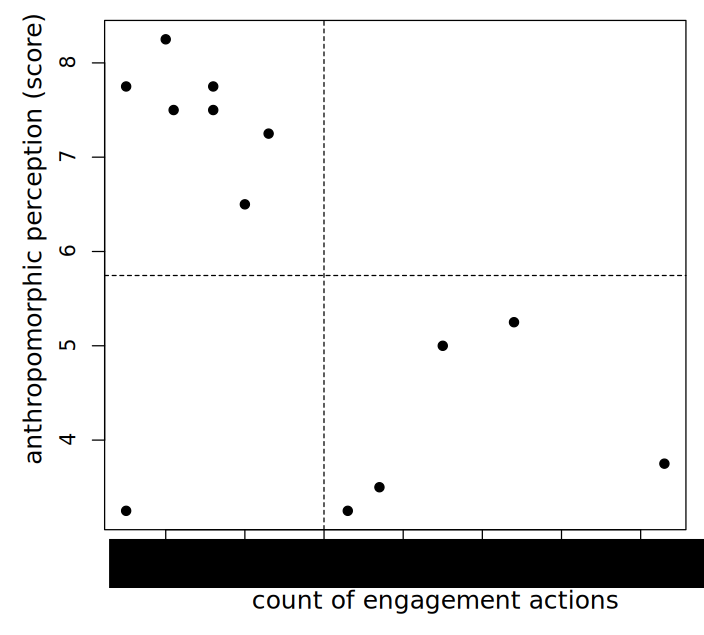
\includegraphics[width=0.6\linewidth]{ranger/domino-correlation}
\end{figure}
        \badge{europe_epfl}
\end{frame}
}

%%%%%%%%%%%%%%%%%%%%%%%%%%%%%%%%%%%%%%%%%%%%%%%%%%%%%%%%%%%%%%%%%%%%%%%%%%%%%%%%%

{
    \paper{Kennedy, Lemaignan et al. {\bf Child Speech Recognition in Human-Robot Interaction[...]} HRI 2017}
\begin{frame}{Automatic Speech Recognition with Children}
    \badge{europe_plym}
    \begin{center}
        \includegraphics<1>[width=0.7\linewidth]{speech-reco/record_img}
         
         \only<2>{
             \footnotesize
\begin{tabular}{@{}rcccccccc@{}}
\toprule
\multicolumn{1}{l}{}                                                                        & \multicolumn{2}{c}{\textbf{Google}}                                                               & \multicolumn{2}{c}{\textbf{Bing}}                                                             & \multicolumn{2}{c}{\textbf{Sphinx}}                                                          & \multicolumn{2}{c}{\textbf{Nuance}}                                                 \\
\multicolumn{1}{l}{}                                                                        & \textit{M} LD    & \textit{\% rec.}                                                  & \textit{M} LD   & \textit{\% rec.}                                              & \textit{M} LD    & \textit{\% rec.}                                             & \textit{M} LD    & \textit{\% rec.}                                    \\ \midrule
\begin{tabular}[c]{@{}r@{}}\textbf{fixed}\\ (\textit{n}=34)\end{tabular}                    & {\bf 0.34} & \textit{\begin{tabular}[c]{@{}c@{}}11.8\\ {[}38{]}\end{tabular}}     & 0.64 & \textit{\begin{tabular}[c]{@{}c@{}}0\\ {[}0{]}\end{tabular}}           & 0.68  & \textit{\begin{tabular}[c]{@{}c@{}}0\\ {[}0{]}\end{tabular}}          & 0.76 & \textit{\begin{tabular}[c]{@{}c@{}}0\\ {[}0{]}\end{tabular}} \\ \midrule
\begin{tabular}[c]{@{}r@{}}\textbf{spontaneous}\\ (\textit{n}=222)\end{tabular}             & {\bf 0.39} & \textit{\begin{tabular}[c]{@{}c@{}}6.8\\ {[}17.6{]}\end{tabular}}    & 0.64 & \textit{\begin{tabular}[c]{@{}c@{}}0.5\\ {[}2.4{]}\end{tabular}}       & 0.80  & \textit{\begin{tabular}[c]{@{}c@{}}0\\ {[}0{]}\end{tabular}}          & 0.80 & \textit{\begin{tabular}[c]{@{}c@{}}0\\ {[}0{]}\end{tabular}} \\ \midrule
\begin{tabular}[c]{@{}r@{}}\textbf{spontaneous}\\ clean only\\ (\textit{n}=83)\end{tabular} & {\bf 0.40} & \textit{\begin{tabular}[c]{@{}c@{}}6.0\\ {[}16.9{]}\end{tabular}}    & 0.63 & \textit{\begin{tabular}[c]{@{}c@{}}1.2\\ {[}1.2{]}\end{tabular}}       & 0.78  & \textit{\begin{tabular}[c]{@{}c@{}}0\\ {[}0{]}\end{tabular}}          & 0.78 & \textit{\begin{tabular}[c]{@{}c@{}}0\\ {[}0{]}\end{tabular}} \\ \bottomrule
\end{tabular}

    \textbf{M} LD: mean Levenshtein distance, at word level.
        }
    \end{center}


\end{frame}
}


\end{document}
